% 八个面板的原始曲线、刻度和随机基线原样保留。
\begin{tikzpicture}
\node[anchor=south west,inner sep=0] (plot) at (0,0) {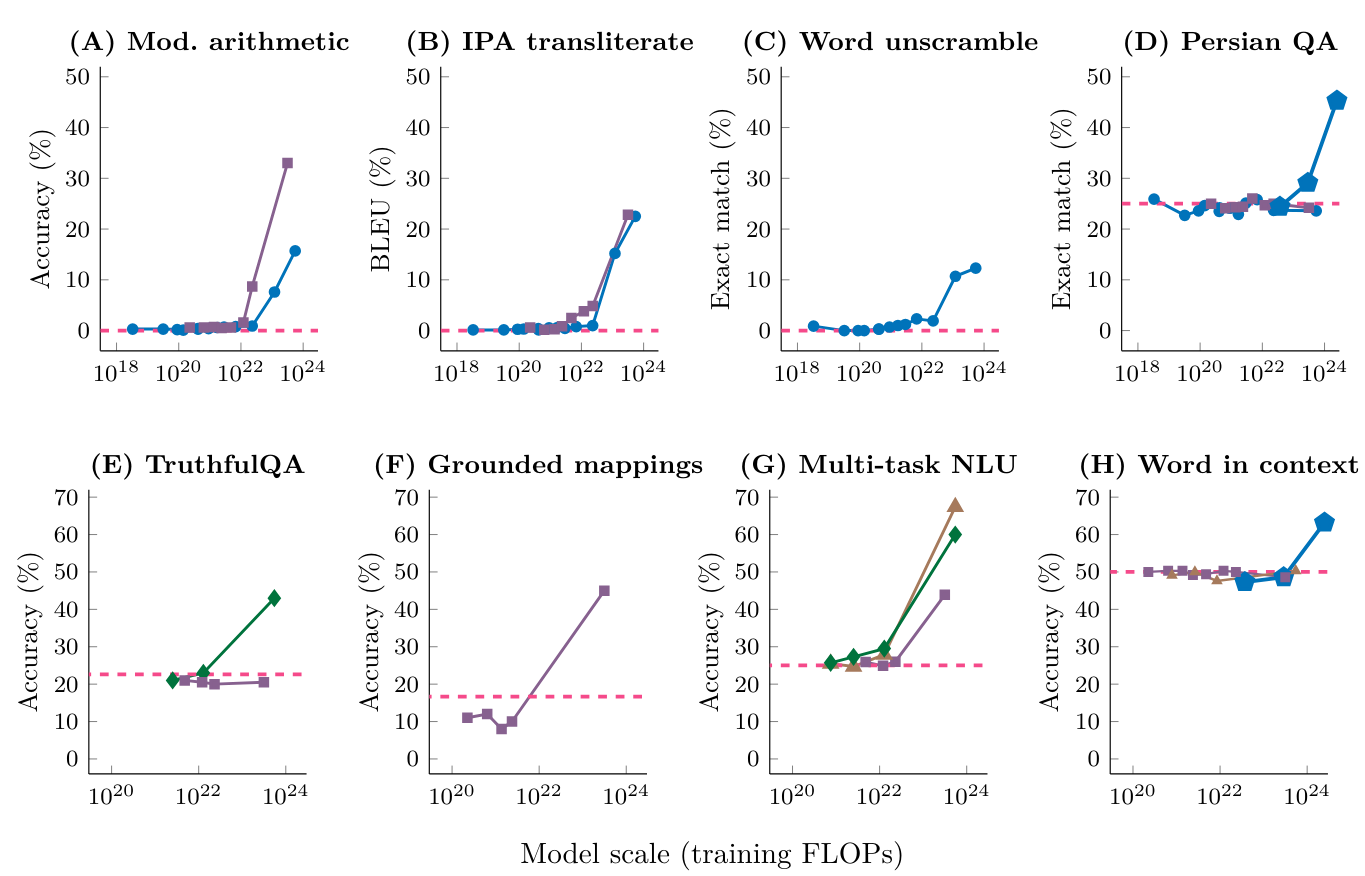
\includegraphics[width=.9\linewidth]{part1/visuals/emergent.png}};
\begin{scope}[x={(plot.south east)},y={(plot.north west)},every node/.style={font=\scriptsize,inner sep=0pt}]
\fill[white] (.04,.935) rectangle (.999,.99);
\node at (.150,.957) {(A) 模算术};
\node at (.404,.957) {(B) 国际音标转写};
\node at (.652,.957) {(C) 字母重排};
\node at (.900,.957) {(D) 波斯语问答};
\fill[white] (.04,.450) rectangle (.999,.492);
\node at (.145,.471) {(E) TruthfulQA};
\node at (.402,.471) {(F) 锚定映射};
\node at (.652,.471) {(G) 多任务自然语言理解};
\node at (.900,.471) {(H) 语境词义};
\foreach \xx/\txt in {.027/准确率（\%）,.278/BLEU（\%）,.528/精确匹配率（\%）,.778/精确匹配率（\%）}{
    \fill[white] (\xx-.015,.59) rectangle (\xx+.015,.86);
    \node[rotate=90] at (\xx,.727) {\txt};
}
\foreach \xx in {.019,.274,.525,.775}{
    \fill[white] (\xx-.015,.12) rectangle (\xx+.015,.39);
    \node[rotate=90] at (\xx,.255) {准确率（\%）};
}
\fill[white] (.34,0) rectangle (.68,.049);
\node at (.51,.024) {模型规模（训练 FLOPs）};
\end{scope}
\end{tikzpicture}
